 \chapter{Tổng quan và mô tả nghiệp vụ}\label{chap:introduction}
	
	Nhu cầu vận chuyển hàng hóa đã có từ rất lâu. Cách thức vận chuyển hàng hóa phổ biến trước đây là thông qua đường bưu điện. Tuy vậy, trong thời đại 4.0 này thì hầu hết mọi dịch vụ đều đang được tự động hóa. Dịch vụ vận chuyển hàng hóa cũng không phải là ngoại lệ. Hiện nay có rất nhiều hệ thống vận chuyển hàng hóa đã được xây dựng. Chẳng hạn ở trong nước có thể kể đến Giao hàng nhanh, Giao hàng tiết kiệm vv... và ở ngoài nước là FedEx hay DHL. Những hệ thống hỗ trợ tự động hóa qui trình logistic và giao nhận hàng hóa là không ít. Tuy vậy việc có thêm một hệ thống sẽ giúp cho người dùng có nhiều lựa chọn để cân nhắc phù hợp với bản thân. Đặc biệt hệ thống nhóm xây dựng sẽ đào sâu hơn về quá trình vận chuyển hàng hóa
	\textbf{liên tỉnh}, tập trung vào những đơn hàng và kiện hàng có khối lượng lớn.\\
	
	Đề tài sẽ được thực hiện trên nền tảng web. Ứng dụng web app sẽ cung cấp các dịch vụ để quy trình vận chuyển hàng hóa liên tỉnh trở nên dễ dàng hơn cho người gửi/nhận, tài xế, thủ kho và quản lí.\\
	
	Ứng dụng sẽ bắt đầu từ việc người dùng gửi yêu cầu muốn giao món hàng bằng cách điền các thông tin cần thiết trên website hệ thống (Tên, địa chỉ bên gửi/nhận, chủ yếu bên nhận và bên gửi sẽ khác tỉnh và cách nhau xa). Sau đó, tài xế sẽ được hệ thống phân công đến những nơi lấy hàng theo yêu cầu bên gửi và tiến hành đi lấy hàng đến khi đầy xe.\\
	
	Sau đó, tài xế sẽ trở lại kho tập trung và gỡ hàng ra đặt trong kho. Quá trình này sẽ được lặp lại cho đến khi tổng hàng hóa thu gom về kho có thể chất đầy một xe container để tiến hành vận chuyển những kiện hàng đó đi liên tỉnh. Xe container đấy sẽ đi xuyên tỉnh và đến kho tập trung ở tỉnh ấy, gỡ hàng ra và sẽ có xe nội thành chuyển trực tiếp đến người nhận theo yêu cầu. Bên liên quan trong từng giai đoạn sẽ trực tiếp cập nhật tình trạng của đơn hàng để người dùng có thể lấy mã đơn hàng và xem trạng thái hiện tại của nó (Đang chờ, đang giao hàng, hoàn thành, etc.). Mỗi khi hàng được chuyển giao đều sẽ có biên bản giao nhận hàng được tạo ra cho mỗi bên.
	
	\begin{figure}[!ht]
		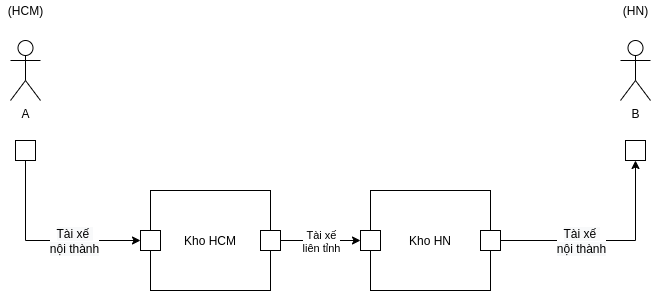
\includegraphics[width=1\textwidth]{/Summary.png}
		\centering
		\linebreak
		\caption{Luồng cơ bản giao nhận hàng hóa}
	\end{figure}
	\newpage
	
	
	\newpage